\documentclass[11pt,a4paper]{article}

\usepackage{main}
\usepackage{cours}

\renewcommand{\typedocument}{Cours}
\renewcommand{\classe}{3e}
\renewcommand{\titre}{Mouvement}

\begin{document}

\pagination

\creertitre{Force et interaction}

\partie{Les actions et interactions}

Pour modifier le mouvement d'un objet, il faut qu'une \important{action mécanique} soit exercée sur lui par un autre objet.

Lorsqu'un objet A exerce une action sur un objet B, B exerce en retour une action opposée sur A (action réciproque). On parle alors d'\important{interaction entre A et B}.

Il existe les \important{interactions de contact} qui se font par contact entre des objets, et les \important{interactions à distance} qui se font à distance (sans contact).

\exemple{Différentes interactions à distance :
    \begin{itemize}
        \item L'interaction \textbf{gravitationnelle}, entre des objets avec une masse.
        \item L'interaction \textbf{magnétique}, entre des objets aimantables ou aimantés.
        \item L'interaction \textbf{électrostatique}, entre des objets chargés électriquement.
    \end{itemize}
}
\vspace{3pt}

Une interaction peut être \important{attractive} (les objets se rapprochent) ou \important{répulsive} (les objets s'éloignent).

Une action est dite \important{localisée} si elle s’exerce sur une petite zone de l’objet, ou \important{répartie} si elle s’exerce sur une grande surface de l’objet.

\exemple{
\begin{itemize}
    \item L'action d'un club sur une balle de golf est \textbf{de contact}, \textbf{répulsive} et \textbf{localisée}.
    \item L'action de la Terre sur la Lune est \textbf{à distance}, \textbf{attractive} et \textbf{répartie} (interaction gravitationnelle).
\end{itemize}
}

Un \important{diagramme objets-interactions} est la représentation d'un objet étudié et de ses interactions avec les objets de son environnement.

\begin{center}
    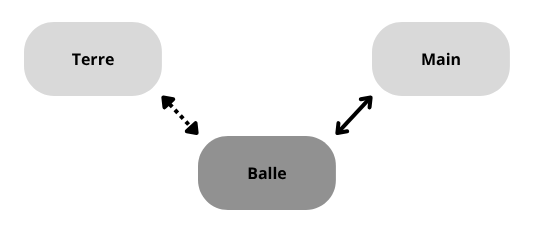
\includegraphics[width=13cm]{images/doi.png}
\end{center}

\exemple{Diagramme objets-interactions d'une balle lancée à la main.\\
Interaction de contact entre la main et la balle, interaction à distance entre la Terre et la balle.}

Les objets sont représentés par des \textbf{rectangles} ou des bulles, les interactions de contact par des \textbf{doubles flèches pleines} et les interactions à distance par des \textbf{doubles flèches en pointillés}. 

\newpage

\partie{Les forces}

\souspartie{Définition}

Une \important{force} représente l'action d'un objet A sur un objet B. On l'écrit \important{$F_{A/B}$} ou \important{$F_{A \rightarrow B}$}.

La force est une \textbf{grandeur physique}, dont l'unité est le \important{Newton (N)}.

On mesure une force avec un \important{dynamomètre}.

\souspartie{Représentation}

Dans un schéma, on représente une force à l'aide d'une \important{flèche} (vecteur) qui a 4 caractéristiques :
\begin{itemize}
    \item Un \important{point d'application} (là où s'exerce la force),
    \item Une \important{direction} ou \textbf{droite d'action} (horizontale, verticale, oblique),
    \item Un \important{sens} (vers le haut/bas, vers la droite/gauche),
    \item Une \important{valeur}, exprimée en Newton. La longueur de la flèche est proportionnelle à la valeur de la force.
\end{itemize}

% Exemple

\souspartie{Effets d'une force sur un objet}

Une force peut produire plusieurs effets sur un objet :
\begin{itemize}
    \item le \textbf{mettre en mouvement},
    \item[] \exemple{On tire dans une balle}
    \item \textbf{modifier sa trajectoire et/ou sa vitesse},
    \item[] \exemple{La balle rebondit sur un obstacle}
    \item \textbf{modifier sa forme}.
    \item[] \exemple{Le pied déforme la balle en la frappant}
\end{itemize}

\vspace{6pt}

Un objet est en \important{équilibre (immobile)} lorsqu'il est soumis à \textbf{deux forces qui se compensent} : elles doivent avoir la même direction, la même valeur, mais des sens opposés.

\begin{center}
    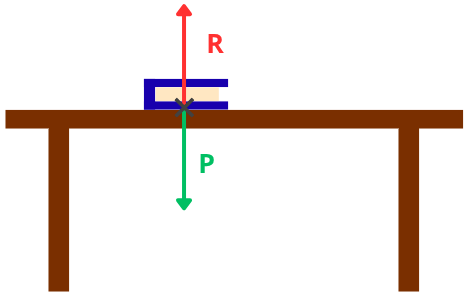
\includegraphics[width=9cm]{images/livre.png}
\end{center}

\exemple{Un livre est posé sur une table.\\
Il est soumis à la force de son propre poids \textbf{P}, verticale et vers le bas, ainsi qu'à la réaction de la table \textbf{R}, perpendiculairement à la surface, donc verticale et vers le haut.\\
Le livre est immobile, les deux forces se compensent et ont la même valeur, donc les deux flèches ont la même taille.}

\newpage

\partie{La gravitation}

La \important{gravitation} est une interaction \textbf{attractive à distance} entre deux objets possédant une masse. Elle \important{augmente avec les masses} des objets et \important{diminue lorsque la distance entre eux augmente}.

On modélise cette interaction par la \important{force gravitationnelle}. Deux objets A et B de masses $m_A$ et $m_B$, séparés d'une distance $d$ exercent l'un sur l'autre une force d'attraction dont la valeur est donnée par la relation :

\begin{center}
    \LARGE\textbf{$F_{A \rightarrow B} = G \times \frac{m_A \times m_B}{d^2}$}
\end{center}

où :
\begin{itemize}
    \item $G = 6,67 \times 10^{-11} SI$ est la \textbf{constante gravitationnelle universelle},
    \item $m_A$ et $m_B$ sont les \textbf{masses} des deux objets (en \textbf{kg}),
    \item $d$ est la \textbf{distance} entre les centres des deux objets (en \textbf{m}),
    \item $F_{A \rightarrow B}$ est la \textbf{force gravitationnelle} exercée par A sur B (en \textbf{N}). Elle est égale à $F_{B \rightarrow A}$.
\end{itemize}

\begin{center}
    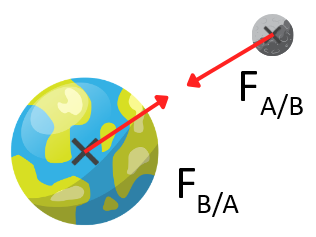
\includegraphics[width=6cm]{images/terre-lune.png}
\end{center}

\exemple{Ici, A est la Terre et B est la Lune.\\[3pt]
Masse de la Terre : $m_A= 5,97 \times 10^{24} \SI{}{\kilogram}$\\
Masse de la Lune : $m_B = 7,36 \times 10^{22} \SI{}{\kilogram}$\\
Distance entre la Terre et la Lune : $d = 3,84 \times 10^{8} \SI{}{\meter}$\\[3pt]
$F_{A/B} = G \times \frac{m_A \times m_B}{d^2} = 6,67 \times 10^{-11} \times \frac{5,97 \times 10^{24} \times 7,36 \times 10^{22}}{(3,84 \times 10^{8})^2} \approx 2 \times 10^{20} \SI{}{\newton} $\\
La valeur de la force gravitationnelle exercée par la Terre sur la Lune est $F_{A/B}=2\times10^{20} \SI{}{\newton}$.\\
Elle est égale à $F_{B/A}$, la valeur de la force exercée par la Lune sur la Terre.
}

\newpage

\partie{Exemples de forces}

\souspartie{Le poids}

Lorsqu'un objet est lâché, il tombe : c'est l'effet de l'action d'attraction de la Terre sur cet objet. Cette force s'appelle le \important{poids}.

Le poids est un cas particulier de la \textbf{force gravitationnelle} : c'est la force exercée par une planète sur un objet situé à sa surface ou à proximité.

Le poids est caractérisé par :
\begin{itemize}
    \item un point d'application \textbf{au centre de gravité} de l'objet.
    \item une direction \textbf{verticale},
    \item un sens \textbf{vers le bas} (vers le centre de la Terre),
\end{itemize}
\vspace{6pt}

Le \textbf{poids est proportionnel à la masse}. Sa valeur est donnée par la relation :

\begin{center}
    \LARGE\important{$P = m \times g$}
\end{center}

où :
\begin{itemize}
    \item $m$ est la \important{masse de l'objet (en kg)} : c'est la quantité de matière contenue dans l'objet, elle est \textbf{invariable} quel que soit l'endroit où l'on se trouve,
    \item $g$ est l'\important{intensité de la pesanteur (en N/kg)} : elle dépend de la planète considérée. Sur Terre, \textbf{$g \approx \SI{9,8}{\newton / \kilogram}$},
    \item $P$ est le \important{poids (en N)}, il dépend aussi de la planète.
\end{itemize}
\vspace{6pt}

\exemple{Reprenons l'exemple du livre donné plus tôt :\\[3pt]
Masse du livre : $m = \SI{0,450}{\kilogram}$\\
Intensité de la pesanteur sur Terre : $g = \SI{9,8}{\newton / \kilogram}$\\[3pt]
$P = m \times g = 0,450 \times 9,8 = \SI{4,41}{\newton}$\\
Le poids du livre est $P= \SI{4,41}{\newton}$.
}

\souspartie{La réaction normale du support}

Lorsqu'un objet repose sur un support, ce support exerce en retour une force sur l'objet : c'est la \important{réaction normale du support}.

Cette force est caractérisée par :
\begin{itemize}
    \item un point d'application \textbf{au point de contact entre l'objet et le support},
    \item une direction \textbf{perpendiculaire} à la surface de contact,
    \item un sens \textbf{opposé} à l'appui de l'objet sur le support (elle "repousse" l'objet).
\end{itemize}
\vspace{6pt}

\exemple{Toujours avec l'exemple du livre, l'intensité de la réaction de la table est égale au poids du livre qu'elle compense, donc $R = \SI{4,41}{\newton}$}

\end{document}